
\paragraph{4. Do new relations introduce new observable behaviors?}
    In any candidate execution, reordering events $e$ and $d$ eliminates the relation $\reln{e}{hb}{d}$ and introduces the new relation $\reln{d}{hb}{e}$. 
    New behaviours created by the latter directly, if any, are 
    of course intentional (and should normally be avoided by ensuring $e$ and $d$ are independent), but we need to ensure that this does not also result in new behaviours indirectly. 
    
    On observing the role on the axioms on this relation, notice that if both $e$ and $d$ are read events then the range does not matter. For all other cases, if events $e$ and $d$ have overlapping ranges, one could introduce a new observable behavior afterreordering them (a simple use of Coherent Reads / Sequentially Consistent Atomics).     

    \critic{blue}{We will later show counter examples for each of the cases that we discard as invalid to reorder.}
    
    Any other new relations that are introduced can be divided into 4 cases, in terms of our events $e$ and $d$ and the newrelation with some event $k$:
    %Show a figure here summarizing the four cases
    \begin{tasks}(2)
        \task  $\et{e}{uo} \ \wedge \ \event{e}{R} \ \wedge \ \reln{k}{hb}{e}$.
        \task  $\et{e}{uo} \ \wedge \  \event{e}{W} \ \wedge \ \reln{k}{hb}{e}$.
        \task  $\et{d}{uo} \ \wedge \  \event{d}{R} \ \wedge \ \reln{d}{hb}{k}$.
        \task  $\et{d}{uo} \ \wedge \ \event{d}{W} \ \wedge \ \reln{d}{hb}{k}$.
    \end{tasks}
    
    \critic{purple}{Change the figure above to represent only the first four cases}
    In each of the above cases, note firstly that we need to only consider cases where their ranges are overlapping/equal.
    
    %Addressing the first case. 
    Figure below shows a breakdown of sub-cases for the first case (a), varying based
    on the nature of event $k$.
    %Show all cases here for different k
    \begin{figure}[H]
        \centering
        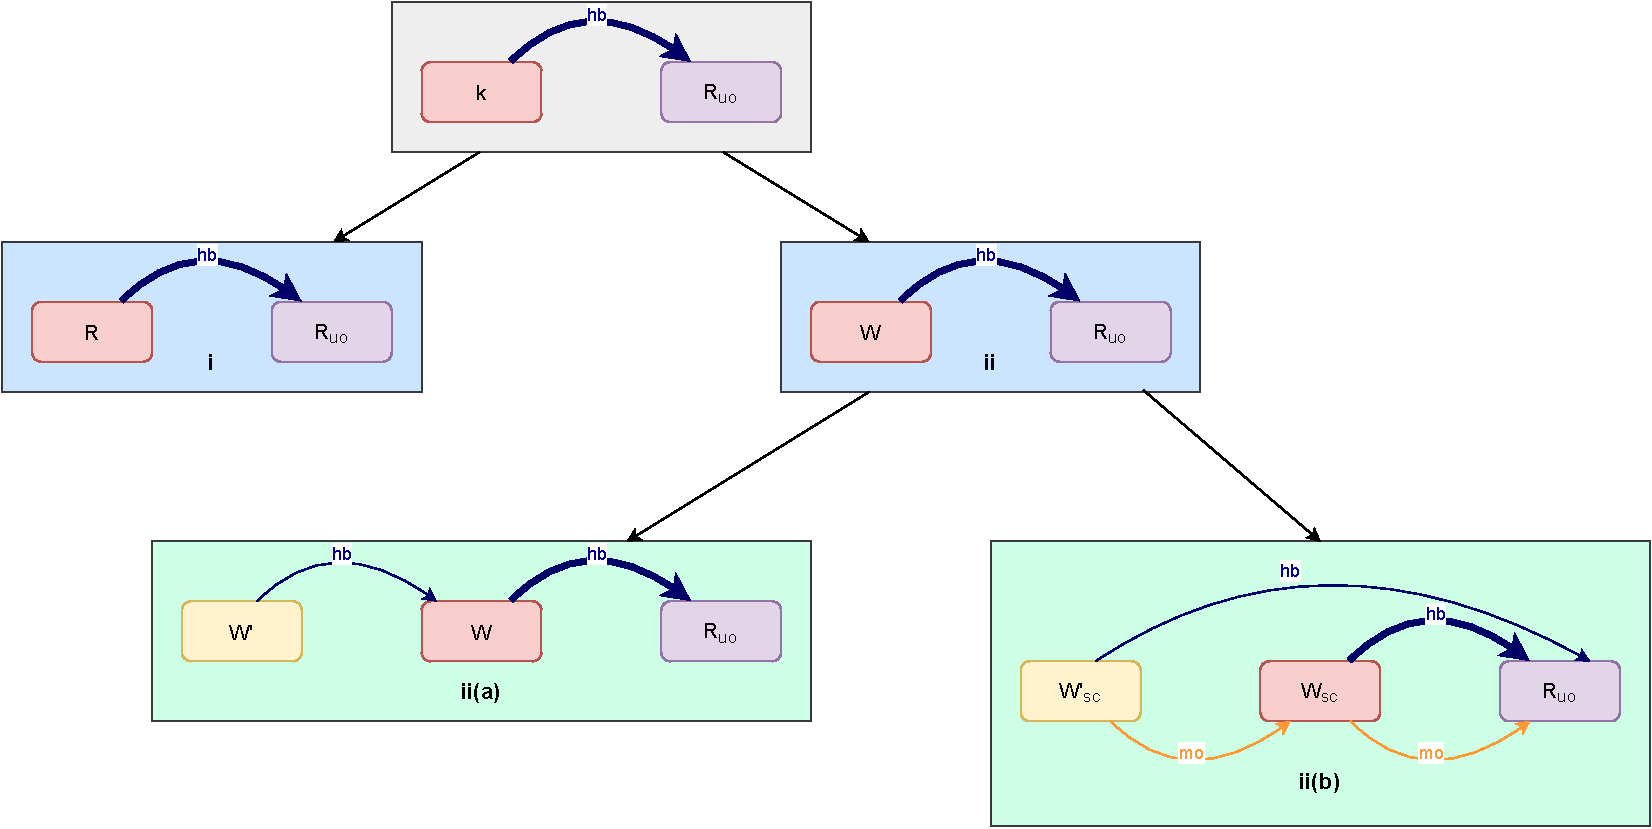
\includegraphics[scale=0.6]{InstructionReordering/ValidReorderingProof/ProofParts/Part4/part4(a).pdf}
        \caption{The role of the axioms on introducing a new relation between an unordered Read and some event $k$}
        \label{fig:my_label}
    \end{figure}
    
    %Might have to elaborate this more
    \begin{enumerate}
        \item For (i), when $k$ is a read, none of the rules have any implications on observable behaviors.
        \item For (ii), when $k$ is a write, the rule of coherent reads (ii(a)) or sequentially consistent atomics (ii(b)) couldrestrict the read ($e$) from reading overlapping ranges of $W'$ with $W$.
    \end{enumerate}
    
    The above case analysis shows us that the new relation could 'trigger' the consistency rules, only to restrict possible reads-from relations, thus restricting possible observable behaviors. 
    The other cases, also have instances which can 'trigger' some cases of the axioms, thus restricting possibly some $\stck{_{rf}}$ relations. These cases are shown in the figures below: 
    \begin{figure}[H]
        \centering
        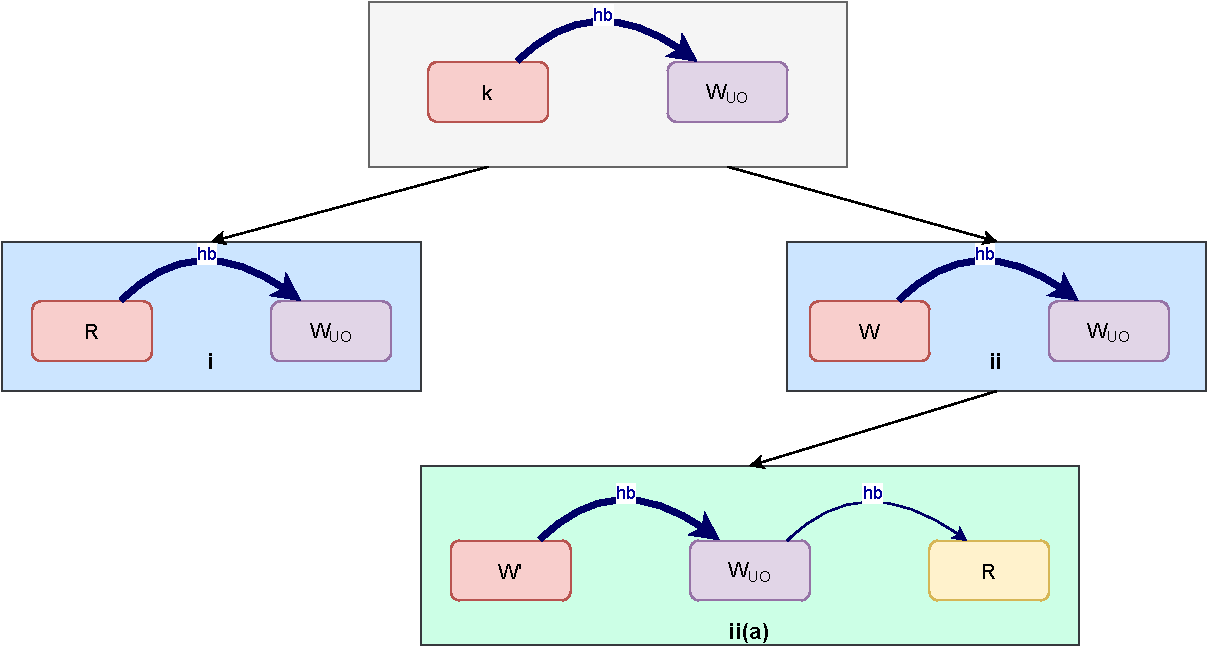
\includegraphics[scale=0.6]{InstructionReordering/ValidReorderingProof/ProofParts/Part4/part4(b).pdf}
        \caption{(i) and (ii(b)) satisfy the axiom of Coherent Reads}
        \label{fig:my_label}
    \end{figure}
          
    \begin{figure}[H]
        \centering
        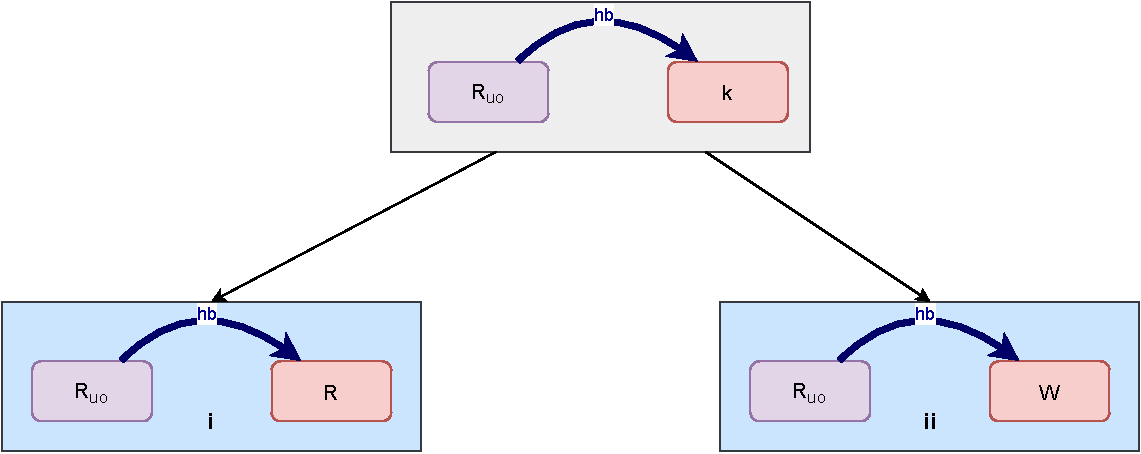
\includegraphics[scale=0.6]{InstructionReordering/ValidReorderingProof/ProofParts/Part4/part4(c).pdf}
        \caption{(ii) satisfies the axiom of Coherent Reads}
        \label{fig:my_label}
    \end{figure}
    
    \begin{figure}[H]
        \centering
        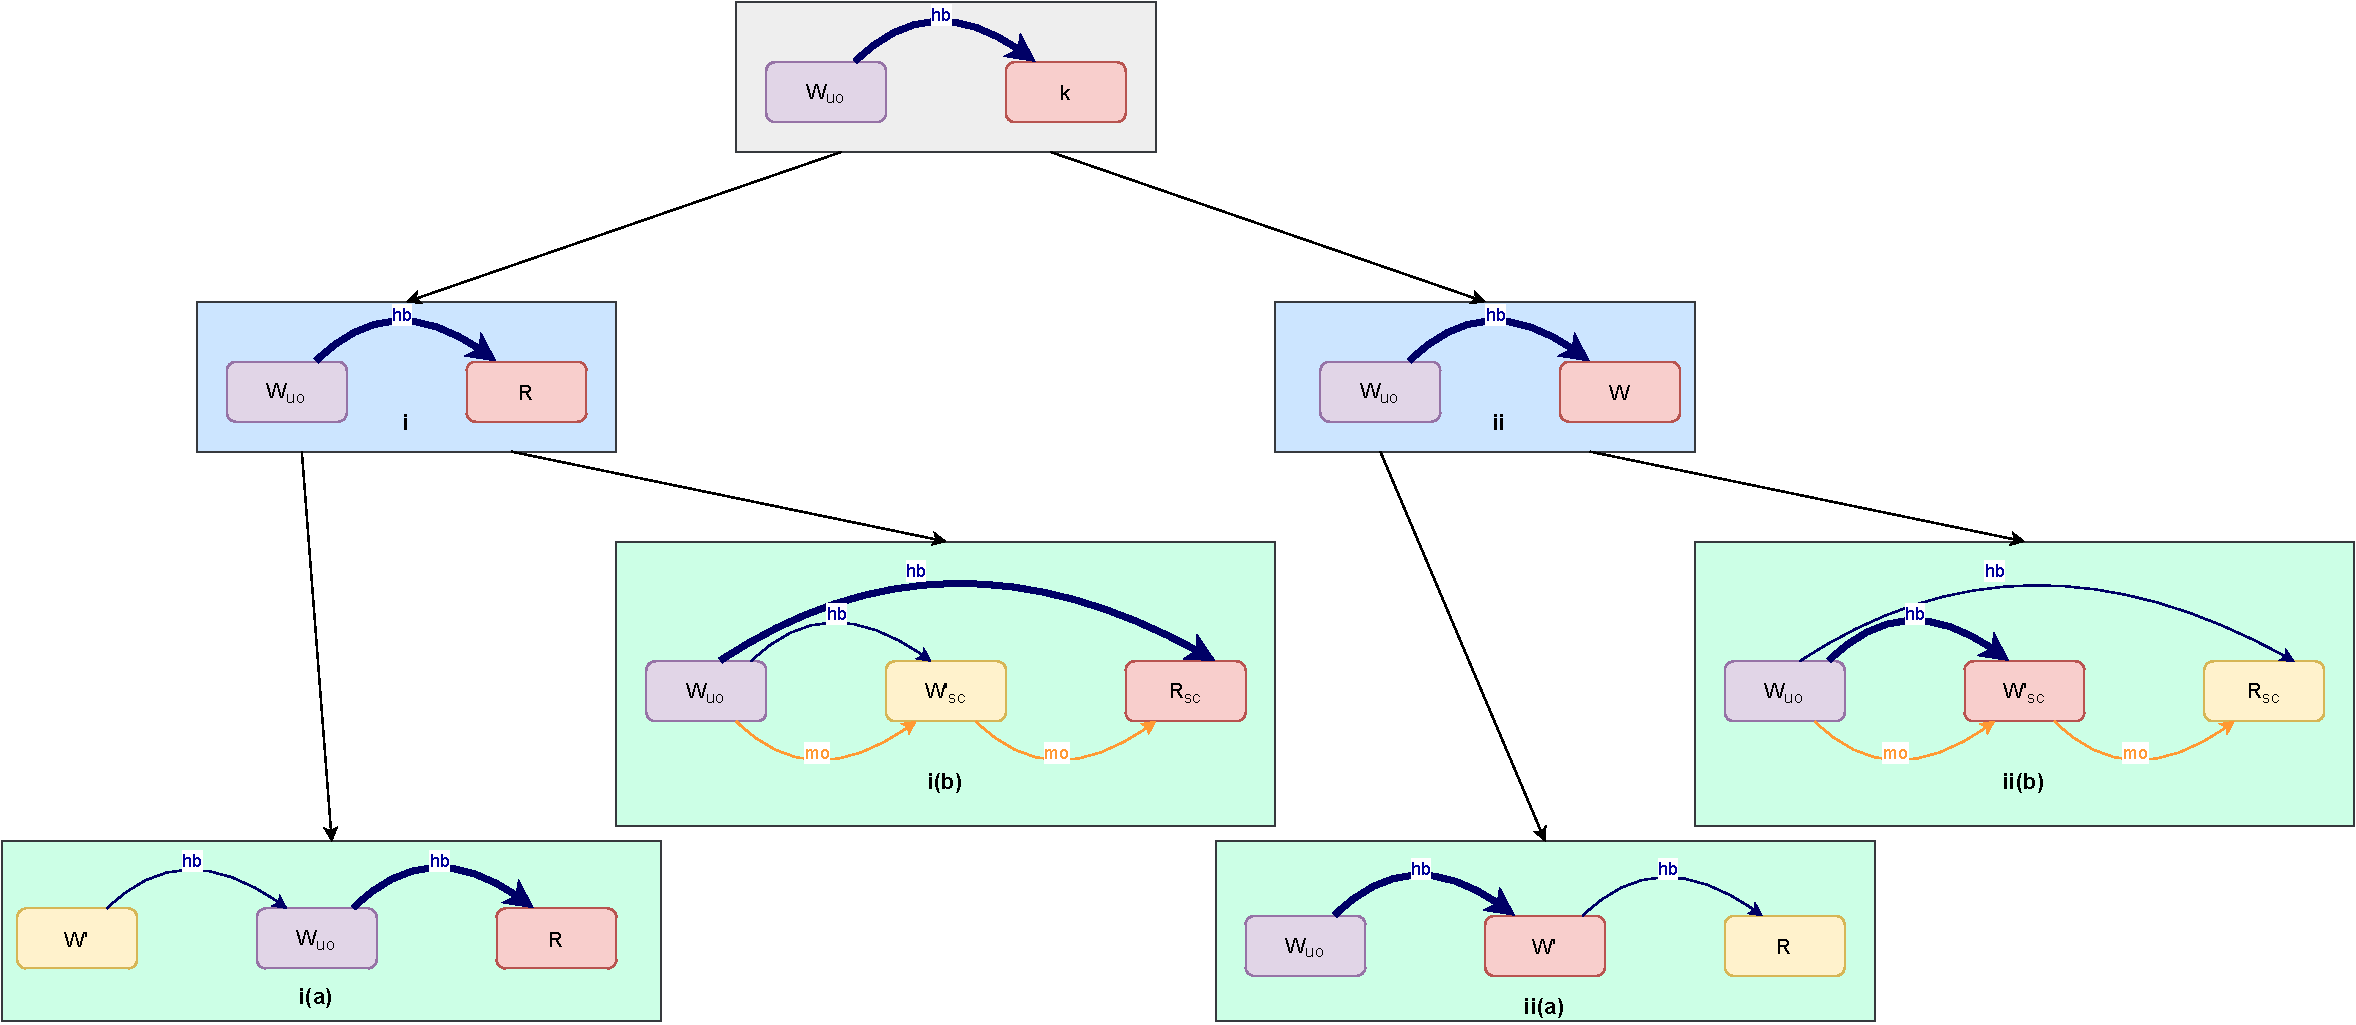
\includegraphics[scale=0.4]{InstructionReordering/ValidReorderingProof/ProofParts/Part4/part4(d).pdf}
        \caption{(i(a)), (ii(a)) satisfy the axiom of Coherent Reads, whereas (i(b)), (ii(b)) satisfy the axiom of SequentiallyConsistent Atomics}
        \label{fig:my_label}
    \end{figure}
    
    \critic{blue}{The main reason for this is that we framed he axioms in a form that restricts \textit{reads-from} relations. Soin any case where adding an additional \textit{happens-before} relation "triggers" an axiom, we are bound to have somebehaviors restricted. It is this fact that is elicited explicitly by going case wise on all relations that are introduced.}
    